%!TEX root = ../thesis.tex
% ******************************* Thesis Appendix B ********************************
\graphicspath{{Appendix2/}}
\chapter{Interface construction, Optimization and ATF calculation on Quantumwise Platform}

\section*{The matching of two surface lattices}
The procedure for matching the two lattices shown as  is as follows:
\begin{itemize}
\item The unit cell vectors of surface $a(a_1,a_2)$ and $b(b_1,b_2)$ are extracted.
\item The $b$ cell is rotated by an angle $\theta$, $(c_1,c_2)$ in
Fig(\ref{fig:cell}).This is done for a set of angles $\theta \in [\theta_{min},\theta_{max}]$ with an default increment $\delta_{\theta}=4$ degrees. For each of the rotations
\begin{itemize}
\item All possible lattice vectors, $v$, where $(c_1,c_2)$ has been repeated a maximun of $()n^{max},m^{max}$ times is found, $v_1 or v_2$ in Fig(\ref{fig:cell})
$$
v=i \times c_1 + j \times c_2,
i \in [-n^{max},n^{max}],j\in [0, m^{max}]
$$
\item We express $v$ in the lattice of cell $a$ by creating a linear transformation
$$
U=\begin{pmatrix} a_{1,x} & a_{2,x} \\ a_{1,y} & a_{2,y} \end{pmatrix},\quad v= Us
$$
where $s=U^{-1}v$ describes how v is expressed in the unit cell vectors $a_1 and a_2$.
\item The vector, v, needs to be truncated to the grid of a. This is done by rounding the elements of s to integers, $s^{'}$, and calculating 
$$
u= U s^{'}
$$
$u(u_1 or u_2 in Fig(\ref{fig:cell}))$ corresponds to the lattice vector of cell $a that v$ will be matched to.
\item All possible cells, $(v_1,v_2)$, of $b$ is created by iterating through all the found lattice vectors $v$ two by two.
\item The strain tensor from the $(v_1,v_2)$ cell to the corresponding $(u_1,u_2)$ cell is calculated. This can be done using the following three straining methods; only straining$(v_1,v_2)$,only straining $(u_1,u_2)$, or straining both equally. For the first straining method, we get
$$
\varepsilon_{11}=|\frac{v_{1,x}}{u_{1,x}}|-1
$$
$$
\varepsilon_{22}=|\frac{v_{2,y}}{u_{2,y}}|-1
$$
$$
\varepsilon_{12}=\frac{1}{2}\frac{v_{2,x}-\frac{u_{1,x}}{u_1,x}u_{2,x}}{u_{2,y}}
$$
Equivalent formulas are used for the second straining method. If both surfaces should be strained equally, an intermediate cell is created between the $(v_1,v_2)$ and $(u_1,u_2)$ cell. This cell in constructed s.t. the strain tensor from the first lattice to the intermediate one is exactly minus the stress tensor from the second to the intermediate one. From the stress tensor, we find the mean absolute stress $\varepsilon^{av}$
$$
\varepsilon^{av}=\frac{\varepsilon_{11}+\varepsilon_{22}+\varepsilon_{12}}{3}
$$
Lattices with a mean absolute stress outside the specified limits $\varepsilon^{av} \in [\varepsilon_{min},\varepsilon_{max}]$ are discarded and strains within a specified \textbf{$tolerance$} are considered equal.
\item The total number of atoms in the corresponding interface is found by considering the area of the cell and the lattice match is ranked according to the following score, $S$
$$
S_{\phi} = \sum_{\alpha} 1- 7 e^{-\frac{(\phi - \alpha)^2}{15}}
$$
$$
\alpha \in [15,33,45,60,90,120,150] degrees
$$
$$
S = e^{-\varepsilon^{av} - \frac{A}{10}- S_{\phi}}
$$
where $\phi$ is the angle between the two vectors of the cell, and 
 $A$is the area of the cell. This score favors the cells where the angle between the vectors are close to any of the angles in $\alpha$, the mean absolute strain is low and the area is small. This is based on the assumption that a small unit cell will be energetically favorable and that a low strain will minimize the amount of defects. The score is a subjective number, created to have a default guess for the interface, and is therefore not meant as a general way of predicting the most physically sensible interface.
\end{itemize}
\item Finally, the lattice match with the best score will be the default choice of the builder.
\end{itemize}



\begin{figure}[htbp!] 
\centering    
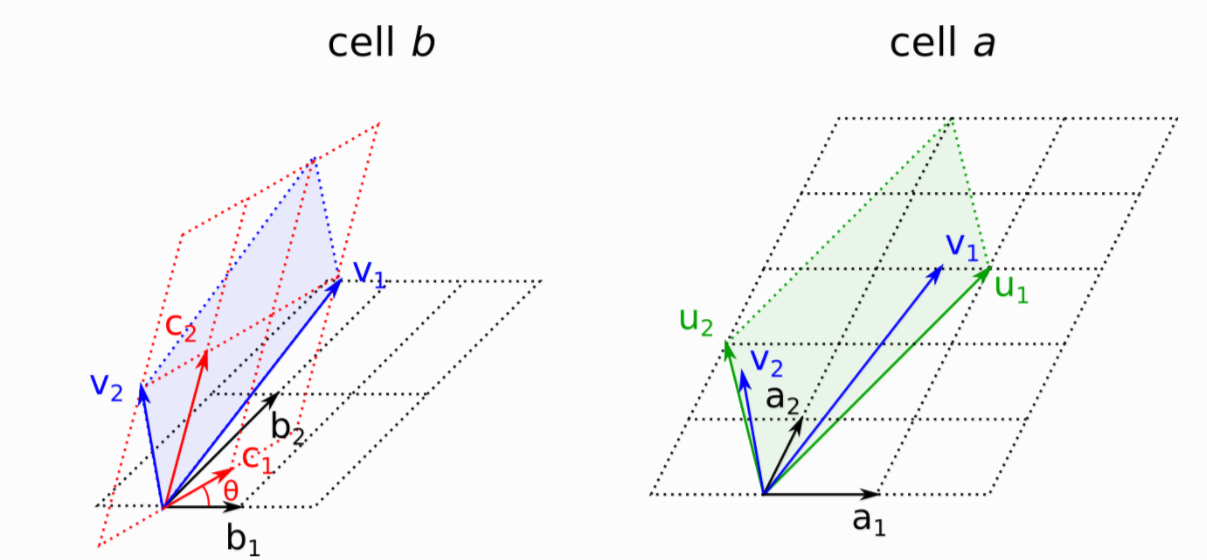
\includegraphics[width=0.6\textwidth]{cell}
\caption[Cell]{Schematic diagram for a general contact-device-contact setup\footnote{From Quantumwise.com}}
\label{fig:cell}
\end{figure}

\section*{Geometry optimization}
Relaxation of the internal coordinates of device configurations can be a tedious and time consuming task. There are two main reasons for this:
\begin{enumerate}
\item The 2-probe configuration consists of three distinct regions: Two electrodes and a central region consisting of electrode extensions and a scattering region. The geometry of each region should be separately optimized in a first-principles manner, but both electrode extensions in the central region must always match the corresponding electrode.
\item The optimum length of the central region is usually not known a priori. In the case of a periodic bulk, one would minimize the stress tensor. However, the stress field is not uniquely defined for a device configuration, so another approach is needed.
\end{enumerate}
\begin{figure}[htbp!] 
\centering    
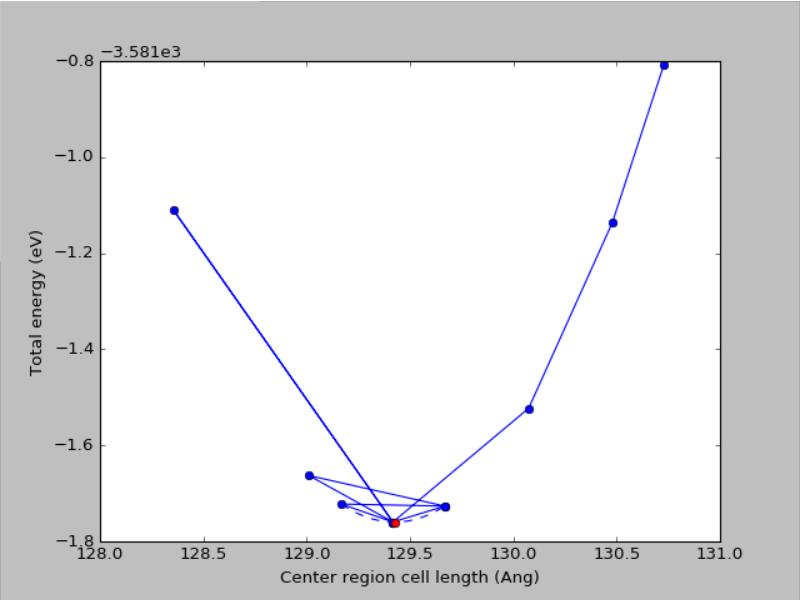
\includegraphics[width=0.6\textwidth]{optimize}
\caption[optimize]{The process of finding the central region length}
\label{fig:optimize}
\end{figure}
We must therefore rely on minimizing the device total energy while explicitly preserving the internal coordinates of the electrode extensions.Based on the $VNL$\footnote{Virtual NanoLab version 2017.0, QuantumWise A/S (www.quantumwise.com)} and $ATK$\cite{ATK1,ATK2,ATK3,ATK4} the Quantumwise provides, there are mainly two ways to do this:
\begin{enumerate}
\item \textbf{BRR}\\
After building the 2-probe configuration from fully relaxed electrodes, you extract the central region bulk and relax it with "Rigid" constraints on the atoms belonging to the electrode extensions. The device or interface is then reassembled from the relaxed bulk. This is a computationally efficient approach and will usually capture a large fraction of the required geometry relaxation. However, it does not take into account any force contributions from the electrodes, so the reassembled device may not be exactly in the global minimum-energy geometry. Some types of electronic structure calculations may be sensitive to this difference, others may not be. We shall refer to this method as Bulk Rigid Relaxation .
\item \textbf{1DMIN}\\
A somewhat more brute-force approach is to explicitly minimize the device total energy wrt. internal coordinates and the central region length, i.e., do the full 2-probe calculations and vary the central region length. This is a 1D minimization problem with relaxation of the atomic positions at each step, so we shall refer to this method as 1DMIN. We have developed a procedure for doing this as efficiently as possible with ATK, but the computations are in general more demanding than with BRR. It is therefore recommend to use 1DMIN only after pre-relaxing the central region with the BRR method. \\
We use the BRR first to conduct \textbf{Bulk Rigid Relaxation of the interface central region}, and then do \textbf{1DMIN optimization of the pre-relaxed interface using 2-probe calculations}.\\

\end{enumerate}

\noindent To search for the the central region length which corresponds minimum interface total energy,we employ a  simple \href{https://docs.scipy.org/doc/scipy-0.13.0/reference/generated/scipy.optimize.minimize_scalar.html#scipy.optimize.minimize_scalar}{SciPy} minimization procedure, whose python code is \href{https://github.com/chieko-feiyuxiao/Oric/tree/master/InterfaceOptimization}{here}.
As can be shown in Fig(\ref{fig:optimize}), the blue points are total energies of relaxed interface configurations, while the red point indicates the optimum central region length. The optimization routine simply maps out the illustrated potential-energy surface and finds its minimum.



